% The components of the stress-energy tensor in one observer's frame.
\documentclass[tikz,border=1pt]{standalone}
% Shared preamble for the standalone figures: the book's fonts, palette and
% drawing styles. Figures are drawn at their final printed size. A column is
% 3.35in (241pt) wide; a figure across both columns is 7in (505pt) wide.

\usepackage[T1]{fontenc}
\usepackage{newpxtext}
\usepackage[varbb]{newpxmath}
\usepackage[semibold,scale=0.95,lining]{sourcesanspro}
\usepackage{xcolor}
% Palette shared by the book and by the standalone figures in figures/src.
% One main hue (blue), one accent (orange), and a few roles used sparingly.

\definecolor{seblue}{HTML}{1D5B8F}    % headings, worked examples, main curves
\definecolor{seblueDark}{HTML}{123E63}
\definecolor{seorange}{HTML}{DC7A26}  % thought experiments, light and light cones
\definecolor{seteal}{HTML}{1F8577}    % checks, travellers and ships
\definecolor{sered}{HTML}{C0392B}     % negative energy, tension, violations
\definecolor{seviolet}{HTML}{5E548E}  % going deeper
\definecolor{sesand}{HTML}{8C6A3F}    % history
\definecolor{segray}{HTML}{6B7480}    % axes, guides, secondary labels
\definecolor{selight}{HTML}{D5DAE1}   % grids and faint rules

\usepackage{siunitx}
\usepackage{fontawesome5}
\usepackage{tikz}
\usetikzlibrary{arrows.meta,calc,positioning,decorations.pathreplacing,
  decorations.markings,shapes.geometric,fadings,shadings,patterns,3d,
  intersections,backgrounds}
\usepackage{pgfplots}
\pgfplotsset{compat=1.18}
\usepgfplotslibrary{fillbetween,groupplots,colormaps}

\tikzset{
  >={Latex[length=2.1mm,width=1.4mm]},
  every picture/.style={line cap=round, line join=round},
  lbl/.style={font=\sffamily\footnotesize, text=black!85},
  smalllbl/.style={font=\sffamily\scriptsize, text=black!75},
  guide/.style={segray, line width=0.4pt},
  axisline/.style={segray, line width=0.5pt, -{Latex[length=1.7mm,width=1.1mm]}},
  light/.style={seorange, line width=0.9pt},
  lightdash/.style={seorange, line width=0.9pt, dash pattern=on 3pt off 2pt},
  ship/.style={seteal, line width=1.4pt},
  cone/.style={fill=seorange!22, draw=seorange!85!black, line width=0.35pt},
}

\pgfplotsset{
  se axis/.style={
    axis lines=left,
    axis line style={segray, line width=0.5pt, -{Latex[length=1.6mm,width=1.1mm]}},
    tick style={segray, line width=0.4pt},
    major tick length=2.5pt,
    tick label style={font=\sffamily\scriptsize, text=black!75},
    label style={font=\sffamily\footnotesize, text=black!85},
    every axis plot/.append style={line width=1.1pt},
    legend style={font=\sffamily\scriptsize, draw=none, fill=none},
    scaled ticks=false,
    xticklabel={\sansnum{\tick}}, yticklabel={\sansnum{\tick}},
  },
}

% Numbers in figures are set in the sans-serif text font, with a true minus.
\sisetup{mode=text, reset-text-family=false, reset-text-series=false,
  reset-text-shape=false, drop-zero-decimal, group-minimum-digits=5}
% Tick values arrive as long decimals (1.5000000000); parse them first.
\newcommand{\sansnum}[1]{\begingroup\pgfkeys{/pgf/fpu=false}%
  \pgfmathparse{1*(#1)}\num{\pgfmathresult}\endgroup}

\begin{document}
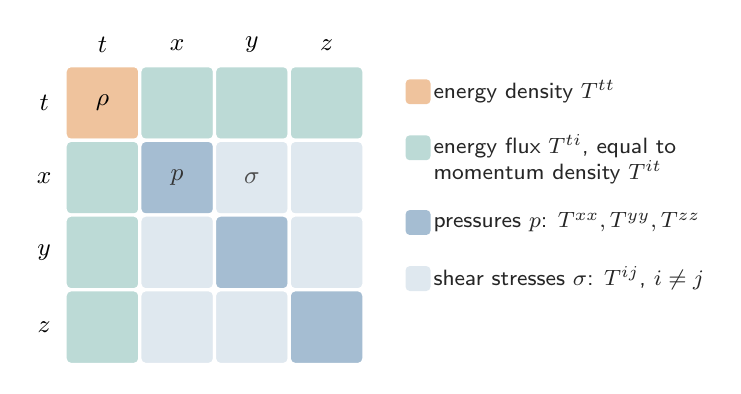
\begin{tikzpicture}[x=27pt, y=27pt,
  cell/.style={rounded corners=2pt, draw=white, line width=1.2pt},
  key/.style={rounded corners=1.5pt, minimum width=9pt, minimum height=9pt, inner sep=0pt},
]
\foreach \i in {0,...,3} \foreach \j in {0,...,3} {
  \ifnum\i=0 \ifnum\j=0 \def\c{seorange!45}\else\def\c{seteal!30}\fi
  \else\ifnum\j=0 \def\c{seteal!30}\else\ifnum\i=\j \def\c{seblue!40}\else\def\c{seblue!14}\fi\fi\fi
  \fill[cell, fill=\c] (\j,-\i) rectangle ++(1,-1);
}
\foreach \l [count=\k from 0] in {t,x,y,z} {
  \node[font=\small] at (\k+0.5,0.28) {$\l$};
  \node[font=\small] at (-0.28,-\k-0.5) {$\l$};
}
\node[font=\small] at (0.5,-0.5) {$\rho$};
\node[font=\small, text=black!80] at (1.5,-1.5) {$p$};
\node[font=\small, text=black!70] at (2.5,-1.5) {$\sigma$};
% key
\begin{scope}[shift={(4.55,-0.35)}, every node/.style={font=\sffamily\footnotesize, anchor=west, text=black!85}]
  \node[key, fill=seorange!45] at (0,0) {}; \node at (0.25,0) {energy density $T^{tt}$};
  \node[key, fill=seteal!30] at (0,-0.75) {}; \node[align=left] at (0.25,-0.9) {energy flux $T^{ti}$, equal to\\momentum density $T^{it}$};
  \node[key, fill=seblue!40] at (0,-1.75) {}; \node at (0.25,-1.75) {pressures $p$: $T^{xx}, T^{yy}, T^{zz}$};
  \node[key, fill=seblue!14] at (0,-2.5) {}; \node at (0.25,-2.5) {shear stresses $\sigma$: $T^{ij}$, $i \ne j$};
\end{scope}
\end{tikzpicture}
\end{document}
